\section{Sphinx Packet Format}

HOPR uses the SPHINX packet format to encapsulate and route data packets in order to provide privacy features such as sender and receiver unlinkability.
Sphinx is a cryptographic message format used to relay anonymized messages within a mix network. A sphinx packet consists of two parts:

\begin{enumerate}
\item Header:
\begin{itemize}
\item Key derivation
\item Routing information
\item Integrity protection
\end{itemize}
\item Body:
\begin{itemize}
\item Onion-Encrypted payload
\end{itemize}
\end{enumerate}
\begin{figure}[H]
    \centering
    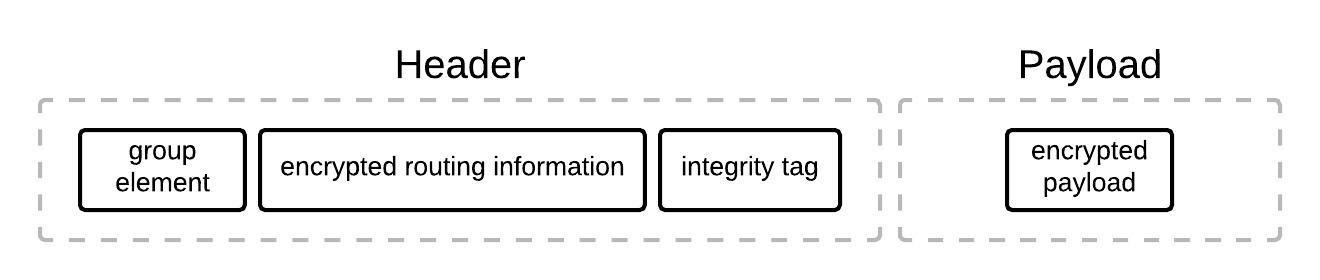
\includegraphics[width=11cm,height=11cm,keepaspectratio]{../yellowpaper/images/sphinx.jpeg}
    \caption{Sphinx packet format}
    \label{fig:Sphinx packet format}
\end{figure}
\subparagraph{Notation:}Let $\kappa=128$ be a security parameter. An adversary will have to do about $2\kappa$ work to break the security of Sphinx with non negligible probability.
Let $r$ be the maximum number of nodes that a Sphinx mix message will traverse before being delivered to its destination. Let $Z$ be  the destination address, an identifier $I \in \{0, 1\}^\kappa$ and a sequence of mix nodes $\{n_0, n_1, . . . , n_{v-1}\}$ with $v\leq r$ the length of the path traversed by the packet. It must also be the case that $|Z| \leq (2(r - v) + 2)$.
\\$G$ is a prime order cyclic group satisfying the Decisional Diffie-Hellman Assumption. The element $g$ is a generator of $G$ and $q$ is the (prime) order of $G$, with $q\approx2^{\kappa}$.
$G^*$is the set of non-identity elements of G. $h_b$is a hash function used to compute blinding factors and we model by random oracles such that:
$h:G^*\times G^*\rightarrow\mathbb{Z}^*_q$ where $\mathbb{Z}^*_q$ is the field of non-identity elements of $\mathbb{Z}_q$ (field of integers).
\\~\\Each node $n$ has a private key $x_n\in \mathbb{Z}^*_q$ and a public key $y_n=g^{x_n}\in G^*$.
The $a_i$ are the group elements which, when combined with the nodes’ public keys, allow computing a shared key for each via Diffie-Hellman (DH) key exchange, and so the first node in the user-chosen route can forward the packet to the next, and only that mix-node can decrypt it.
The $s_i$ are the DH shared secrets, $b_i$ are the blinding factors. $\phi$ is a filler string that is used to ensure the header packets remain constant in size as layers of encryption are added or removed. 

\paragraph{Key derivation}
The sender $(A)$ picks a random $x\in \mathbb{Z}^*_q$ that is used to derive new keys for every packet. 
\newline $(A)$ randomly picks a path consisting of intermediate nodes $(B)$, $(C)$,$(D)$ and the final destination of the packet $(Z)$. 
\newline $(A)$ performs an offline Diffie-Hellman key exchange with each of these nodes and derives shared keys with each of these nodes.
\newline $(A)$ computes a sequence of $r$ tuples (in our case r=4)  $$(a_0,s_0,b_0),.................,(a_{r-1},s_{r-1},b_{r-1})$$ as follows:
\begin{itemize}
\item $a_0=g^x,s_0=y^x_B,b_0=h(a_0,s_0)$
\item $a_1=g^{xb_0},s_1=y^{xb_0}_C,b_1=h(a_1,s_1)$
\item $a_2=g^{xb_0b_1},s_2=y^{xb_0b_1}_D,b_2=h(a_2,s_2)$
\item $a_3=g^{xb_0b_1b_2},s_3=y^{xb_0b_1b_2}_D,b_3=h(a_3,s_3)$
\end{itemize}
 Where $y_B,y_C,y_D,y_Z$ are the public keys of the nodes $B,C, D$  which we assume to be available to $A$ .

\paragraph{Routing information}
Each node on the path needs to know the next downstream node. Therefore, the sender $(A)$ generates routing information $\beta_i$ for $(B)$, $(C)$ and (D) as well as message END to tell $(Z)$ that it is the final receiver of the message. The END message is a distinguished prefix byte (since it isn't an element of $G$) that's added to the final receiver's address.
$$\beta_i=(\Delta\|I\|0_{(2(r-v)+2)\kappa-|\Delta|}\oplus PRNG(s_{v-1})_{[ \,0....(2(r-v)+3)\kappa-1})\|\phi$$
\newline Since $(A)$ has a shared secret with each of the nodes along the path, it is able to derive blindings for each of them. 
\newline Each node along the path receives an authentication tag $\gamma_i$ in the form of a message authentication code (MAC)
which is encoded in the header.
\newline Some padding is added at each mix stage in order to keep the length of the message invariant at each hop. 
\\~\\The mix header is constructed as follow: $$M_i=(a_i,\beta_i,\gamma_i)$$ 
\newline Once $(B)$ receives the packet, it derives the shared key $s_0$ by computing $$s_0=(a_0)^b=(g^x)^b=(g^b)^x=y^x_B$$ and removes its blindings. This allows $(B)$ to unblind the routing info that tells $(B)$ the public key of the next downstream node $(C)$. In order to extract the routing instructions, the mix-node B first appends a zero-byte padding at the end of $\beta_0$ and decrypts the padded block of routing information $B$ by XORing it with $PRNG(s_{v-1})$ as follows:
$$(\beta_0\|0_{2\kappa})\oplus PRNG(s_{v-1})$$
(B) parses the routing instructions from $(A)$ in order to obtain the address of the next mix-node $(C)$, as well the new integrity tag $\gamma_1$ and $\beta_1$, which should be forwarded to the next hop and blinds the key share $a_0=g^x$ by setting it to $a_1=g^{xb_0}$
\paragraph{Integrity check}
By using the derived shared secret $s_i$, each node is able to recompute the authentication tag and check the integrity of the received packet as follows: $$\gamma_i=HMAC(s_i,\beta_i)$$
This integrity check allows to verify whether or not the header was modified.
\paragraph{Encrypt \& Decrypt}
The payload is where the actual message is hidden and is computed in different layers using a block cipher encryption algorithm and is decrypted at each stage of mixing. $(B)$ removes one layer of encryption from the payload $\delta_0$ and sends it to $(C)$ where:
$$\delta_i=\pi^{-1}(h_{\pi}(s_{i-1}), \delta_{i-1})$$
Any attempt of modification by an attacker would result in message distruction and thus is would be irrecoverable. 
\\~\\Same happens at $(C)$ and $(D)$: key derivation, unblinding, deleting, shifting, decryption and blinding. 

\subsection*{Implementation choices}
The implementation choices taken by HOPR team are the following:
\begin{itemize}
    \item \textbf{Cyclic group:} The cyclic group used in the HOPR Sphinx implementation is an elliptic curve group on the Ethereum secp256k1 curve and thus operations will be done on the elliptic curve.
    \item \textbf{Hash function:} BLAKE2s hash function which is a cryptographic hash function faster than SHA-2 and SHA-3, yet is at least as secure as SHA-3 and produces digests of any size between 1 and 32 bytes.
    \item \textbf{MAC:} HMAC based on a hash function BLAKE2s.
    \item \textbf{Encryption scheme:} LIONESS implementation based on the ChaCha20 stream cipher.
    \item \textbf{Padding:} In the original SPHINX paper, a sequence of only 0s is used for padding, this allows the last mix-node in the path to infer information about the length of the path and the last destination, hence breaking one of the security properties promised by Sphinx. In order to prevent this attack, We replace the 0-padding by a randomized padding for the last exit-mix node and always take $v=r$. This way, the exit node can't identify where the padding starts and thus won't be able to find the path length that preceeds the padding.
\end{itemize}





